% Commands

\newcommand{\authorinfo}{Arne Struck, Lars Thoms}
\newcommand{\titleinfo}{AD [HA] zum 4. 12. 2013}
\newcommand{\qed}{\ \square}
\newcommand{\limn}{\lim\limits_{n\to\infty}}
\newcommand{\todo}{\textcolor{red}{\textbf{TODO}}}

% ------------------------------------------------------

% Packages & Stuff

\documentclass[a4paper,11pt,ngerman]{scrartcl}
\usepackage[german,ngerman]{babel}
\usepackage[utf8]{inputenc}
\usepackage[T1]{fontenc}
\usepackage[top=1.3in, bottom=1.2in, left=0.9in, right=0.9in]{geometry}
\usepackage{lmodern}
\usepackage{amssymb}
\usepackage{amsmath}
\usepackage{enumerate}
\usepackage{fancyhdr}
\usepackage{pgfplots}
\usepackage{algorithm}
\usepackage{algorithmicx}
\usepackage{algpseudocode}
\usepackage{multicol}
\usepackage[parfill]{parskip}
\usetikzlibrary{automata,calc,patterns,shapes}


% ------------------------------------------------------

% Title & Pages

\title{\titleinfo}
\author{\authorinfo}

\pagestyle{fancy}
\fancyhf{}
\fancyhead[L]{\authorinfo}
\fancyhead[R]{\titleinfo}
\fancyfoot[C]{\thepage}

\begin{document}
	\maketitle
	\begin{enumerate}
		\item[\textbf{1.}]
		\begin{enumerate}
			\item[a)]\quad \\
				Der Algorithmus funktioniert nicht mehr. Dies wird an folgendem Gegenbeispiel deutlich 
				(gesucht wird 5, die Zeile ist abgeändert):
				\begin{verbatim}
					in: A[int] = [1,2,3,4,5]
					low = 0, high = 4, mid = 2
					A[mid] < 5
					
					low = 2 + 1, high = 4, mid = 3
					A[mid] < 5
					
					low = 3 + 1, high = 4, mid = 4
					
					return not_found
				\end{verbatim}
				Die 5 wird nicht gefunden, da die Bedingung (while low < high) nicht mehr gilt.
			\item[b)]\quad \\
				Die Verarbeitung einer absteigend sortierten Liste lässt sich durch das Invertieren der 
				Vergleichszeichen innerhalb der while-Schleife erreichen, wodurch die Verarbeitung des 
				Algorithmus ''umgedreht'' wird.
				\begin{verbatim}
					BinarySearch(A[0..N-1],value){
					    low = 0;
					    high = N - 1;
					    while(low <= high){
					        mid = (low + high) / 2;
					        if(A[mid] < value){
					            high = mid - 1;
					        }
					        else if (A[mid] > value){
				    	        low = mid + 1;
					        }
					        else{
					            return mid;
					        }
					    }
					    return not_found;
					}
				\end{verbatim}
			\item[c)]\quad \\
				Korrekte Eingaben vorausgesetzt, ist es unumgänglich die while-Schleife zu betreten,
				hier gilt low <= mid <= high. Nun wird die Differenz von low und high pro Iteration um mindestens
				1 verringert, wenn der Algorithmus noch nicht terminiert hat. Die Verringerung der Differenz 
				resultiert aus den beiden Vergleichen. Daraus resultiert, dass nach spätestens n (n  = Array-
				Länge) Iterationen low = mid = high gilt, womit der Wert A[mid] ausgegeben wird. Damit ist bei
				korrekter Eingabe Terminierung garantiert.
			\item[d)]\quad \\
				
		\end{enumerate}
		\item[\textbf{2.}]
		\begin{enumerate}
			\item[a)]
			\begin{enumerate}
				\item[(i)]\quad \\
					Zu zeigen wären 2 Behauptungen:
					\begin{multicols}{2}
						\[E = \emptyset \Rightarrow 1-\text{färbbar}\] \\
						Da keine Kante existiert, besitzt kein Knoten einen Nachbarknoten.
						Also kann auch jeder Knoten in der gleichen Farbe gefärbt werden \\ \\

						\[E = \emptyset \Leftarrow 1-\text{färbbar}\] \\
						Wenn alle Knoten in der gleichen Farbe gefärbt sind, können auch keine Nachbarknoten
						existieren, da diese nicht gleich eingefärbt werden dürfen. Damit ist gezeigt, dass
						im Fall der 1-Färbung keine Kanten existieren können.
					\end{multicols}
				\item[(ii)]\quad \\
					Zu zeigen ist also, wenn eine Abbildung $c_k:V\rightarrow\{1,..,k\}$ existiert muss
					auch eine Abbildung $c_k:V\rightarrow\{1,..,k,k+1\}$ existieren.
					Da $c_k$ nicht surjektiv sein muss, kann jeder Graph trivialer Weise als (k+1)-färbbar 
					angesehen werden (es müssen ja nicht alle Färbungen Anwendung finden).
					Wäre dem nicht so, dann wären injektive Abbildungen ein Problem bei der (k+1)-Färbung.
				\item[(iii)]\quad \\
					Annahme: \(n = |V|\) ($n$ wird nicht genauer spezifiziert) \\
					Für jedes \(n \in V\) wird eine Farbe in \(c_k\) reserviert (wenn $k < n$ gilt, werden neue 
					Farben hinzugefügt). Nun wird eine injektive Abbildung erstellt (bijektiv, wenn zuvor $k < n$ 
					und jetzt $k = n$). Damit ist jedes $n$ einer eigenen Farbe zugeordnet und somit eine 
					$n$-Färbung erreicht.
			\end{enumerate}
			\item[b)]
			\begin{enumerate}
				\item[(i)]\quad \\
					Zu zeigen: \(2-\text{färbbar} \Rightarrow\) bipartit. \\
					Die 2-Färbung bedeutet, dass 2 ''Gruppen'' von Knoten keine direkten Nachbarknoten in der 
					gleichen ''Gruppe'' haben (ansonsten könnten sie nicht gleich gefärbt sein).
					Diese ''Gruppen'' kann man auch als Mengen auffassen. Damit ist die Definition von bipartiten 
					Graphen hergestellt, da diese einen Graphen in 2 Mengen unterteilen, wobei die Elemente der 
					Teilmengen dieser 2 Mengen nicht miteinander durch Kanten verbunden sind.
				\newpage
				\item[(ii)]\quad \\
					\begin{verbatim}
						2colored(V){
						    Set1 = Set;
						    Set2 = Set;
						    color1 = randomElement(V).getcolor();
						    color2 = color1;
						    while(color1 = color2){
						        color2 = randomElement(V).getcolor();
						    }
						    forAll(v in V){
						        if(v.getcolor() = color1){
						            Set1.add(v);
						        }
						        else if (v.getcolor() = color1){
						            Set2.add(v);
						        }
						        else{
						            return no_2color;
						        }
						    }
						    return Set1,Set2;
						}
					\end{verbatim}
				\item[(iii)]\quad \\
					Sofern der Graph zusammenhängend ist (und es sich um eine echte 2-Färbung handelt, also nur
					2 Farben vorhanden sind) existieren 2 mögliche Färbungen (die Farben werden vertauscht). \\
					Ansonsten hängt die Anzahl der Färbungen von der Anzahl der Zusammenhangskomponenten (n) ab.
					Man kann das ganze Problem als Binärbaum auffassen. Die Höhe des Baumes entspricht der Anzahl 
					der Zusammenhangskomponenten. Jede Färbung würde dann einem Blatt entsprechen. \(2^n\) Wäre 
					damit die Anzahl der Blätter in der n-ten Ebene, also bei n Zusammenhangskomponenten.
			\end{enumerate}
			\item[c)]
			\begin{enumerate}
				\item[(i)]\quad \\
				\todo
				\item[(ii)]\quad \\
				\todo
				\item[(iii)]\quad \\
				\todo
				\item[(iv)]\quad \\
				\todo
			\end{enumerate}
		\end{enumerate}
		\item[\textbf{3.}]
		\begin{enumerate}
			\item[a)]\quad
			\begin{description}
				\item[$G_1$] 1, 3, 4, 5, 2, 8, 6, 7
				\item[$G_2$] 1, 3, 5, 6, 4, 2, 7
			\end{description}
			\item[b)]\quad
			\begin{description}
				\item[$G_1$] 4, 3, 1, 7, 6, 8, 2, 5
				\item[$G_2$] 4, 6, 5, 3, 1, 2, 7
			\end{description}
			\item[c)]\quad
			\begin{description}
				\item[$G_1$] 1, 3, 5, 4, 2, 7, 8, 6
				\item[$G_2$] 1, 3, 4, 7, 5, 2, 6
			\end{description}
			\item[d)]\quad
			\begin{description}
				\item[$G_1$] Für diesen Graphen kann keine topologische Sortierung existieren, da er sowohl einen reflexiven Knoten enthält (8, Verstoß gegen die Bedingung der Irreflexität) und mehrere Zyklen enthält ([1,5], [7,8], [1,5,2], ...)
				\item[$G_2$] 1, 7, 2, 3, 5, 6, 4
			\end{description}
			\item[e)]\quad \\
				Die von uns gefundene topologische Sortierung ist nicht eindeutig. Damit eine solche Sortierung eindeutig ist, muss sie einen Hamiltonkreis aufweisen. Dieser Graph kann aber keinen Hamiltonkreis beinhalten, da allein schon der Knoten ''1'' drei ausgehende Kanten besitzt.
			\item[f)]\quad
				\begin{multicols}{2}
					Der Graph ''$G_2$'' besitzt keine starken Zusammenhangskomponenten, da er keinerlei Zyklen aufweist. \\
					Nur der Graph ''$G_1$'' besitzt eine starke Zusammenhangskomponente, die Knoten ''3'' oder ''4'' bilden keine starke Zusammenhangskomponente. \\
					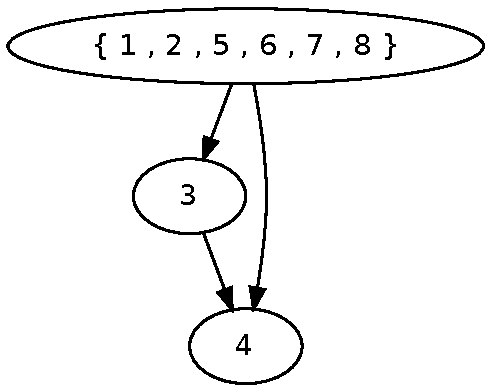
\includegraphics[scale=0.6]{g1.pdf}					
				\end{multicols}
		\end{enumerate}
		\item[\textbf{4.}]
		\begin{enumerate}
			\item[a)]\quad \\
			\todo
			\item[b)]\quad \\
			\todo
			\item[c)]\quad \\
			\todo
		\end{enumerate}
	\end{enumerate}
\end{document}
